\documentclass[../main.tex]{subfiles}
\graphicspath{{\subfix{../img/}}}

\begin{document}

\section{Additional Figures}

\begin{figure}[!b]
    \centering
    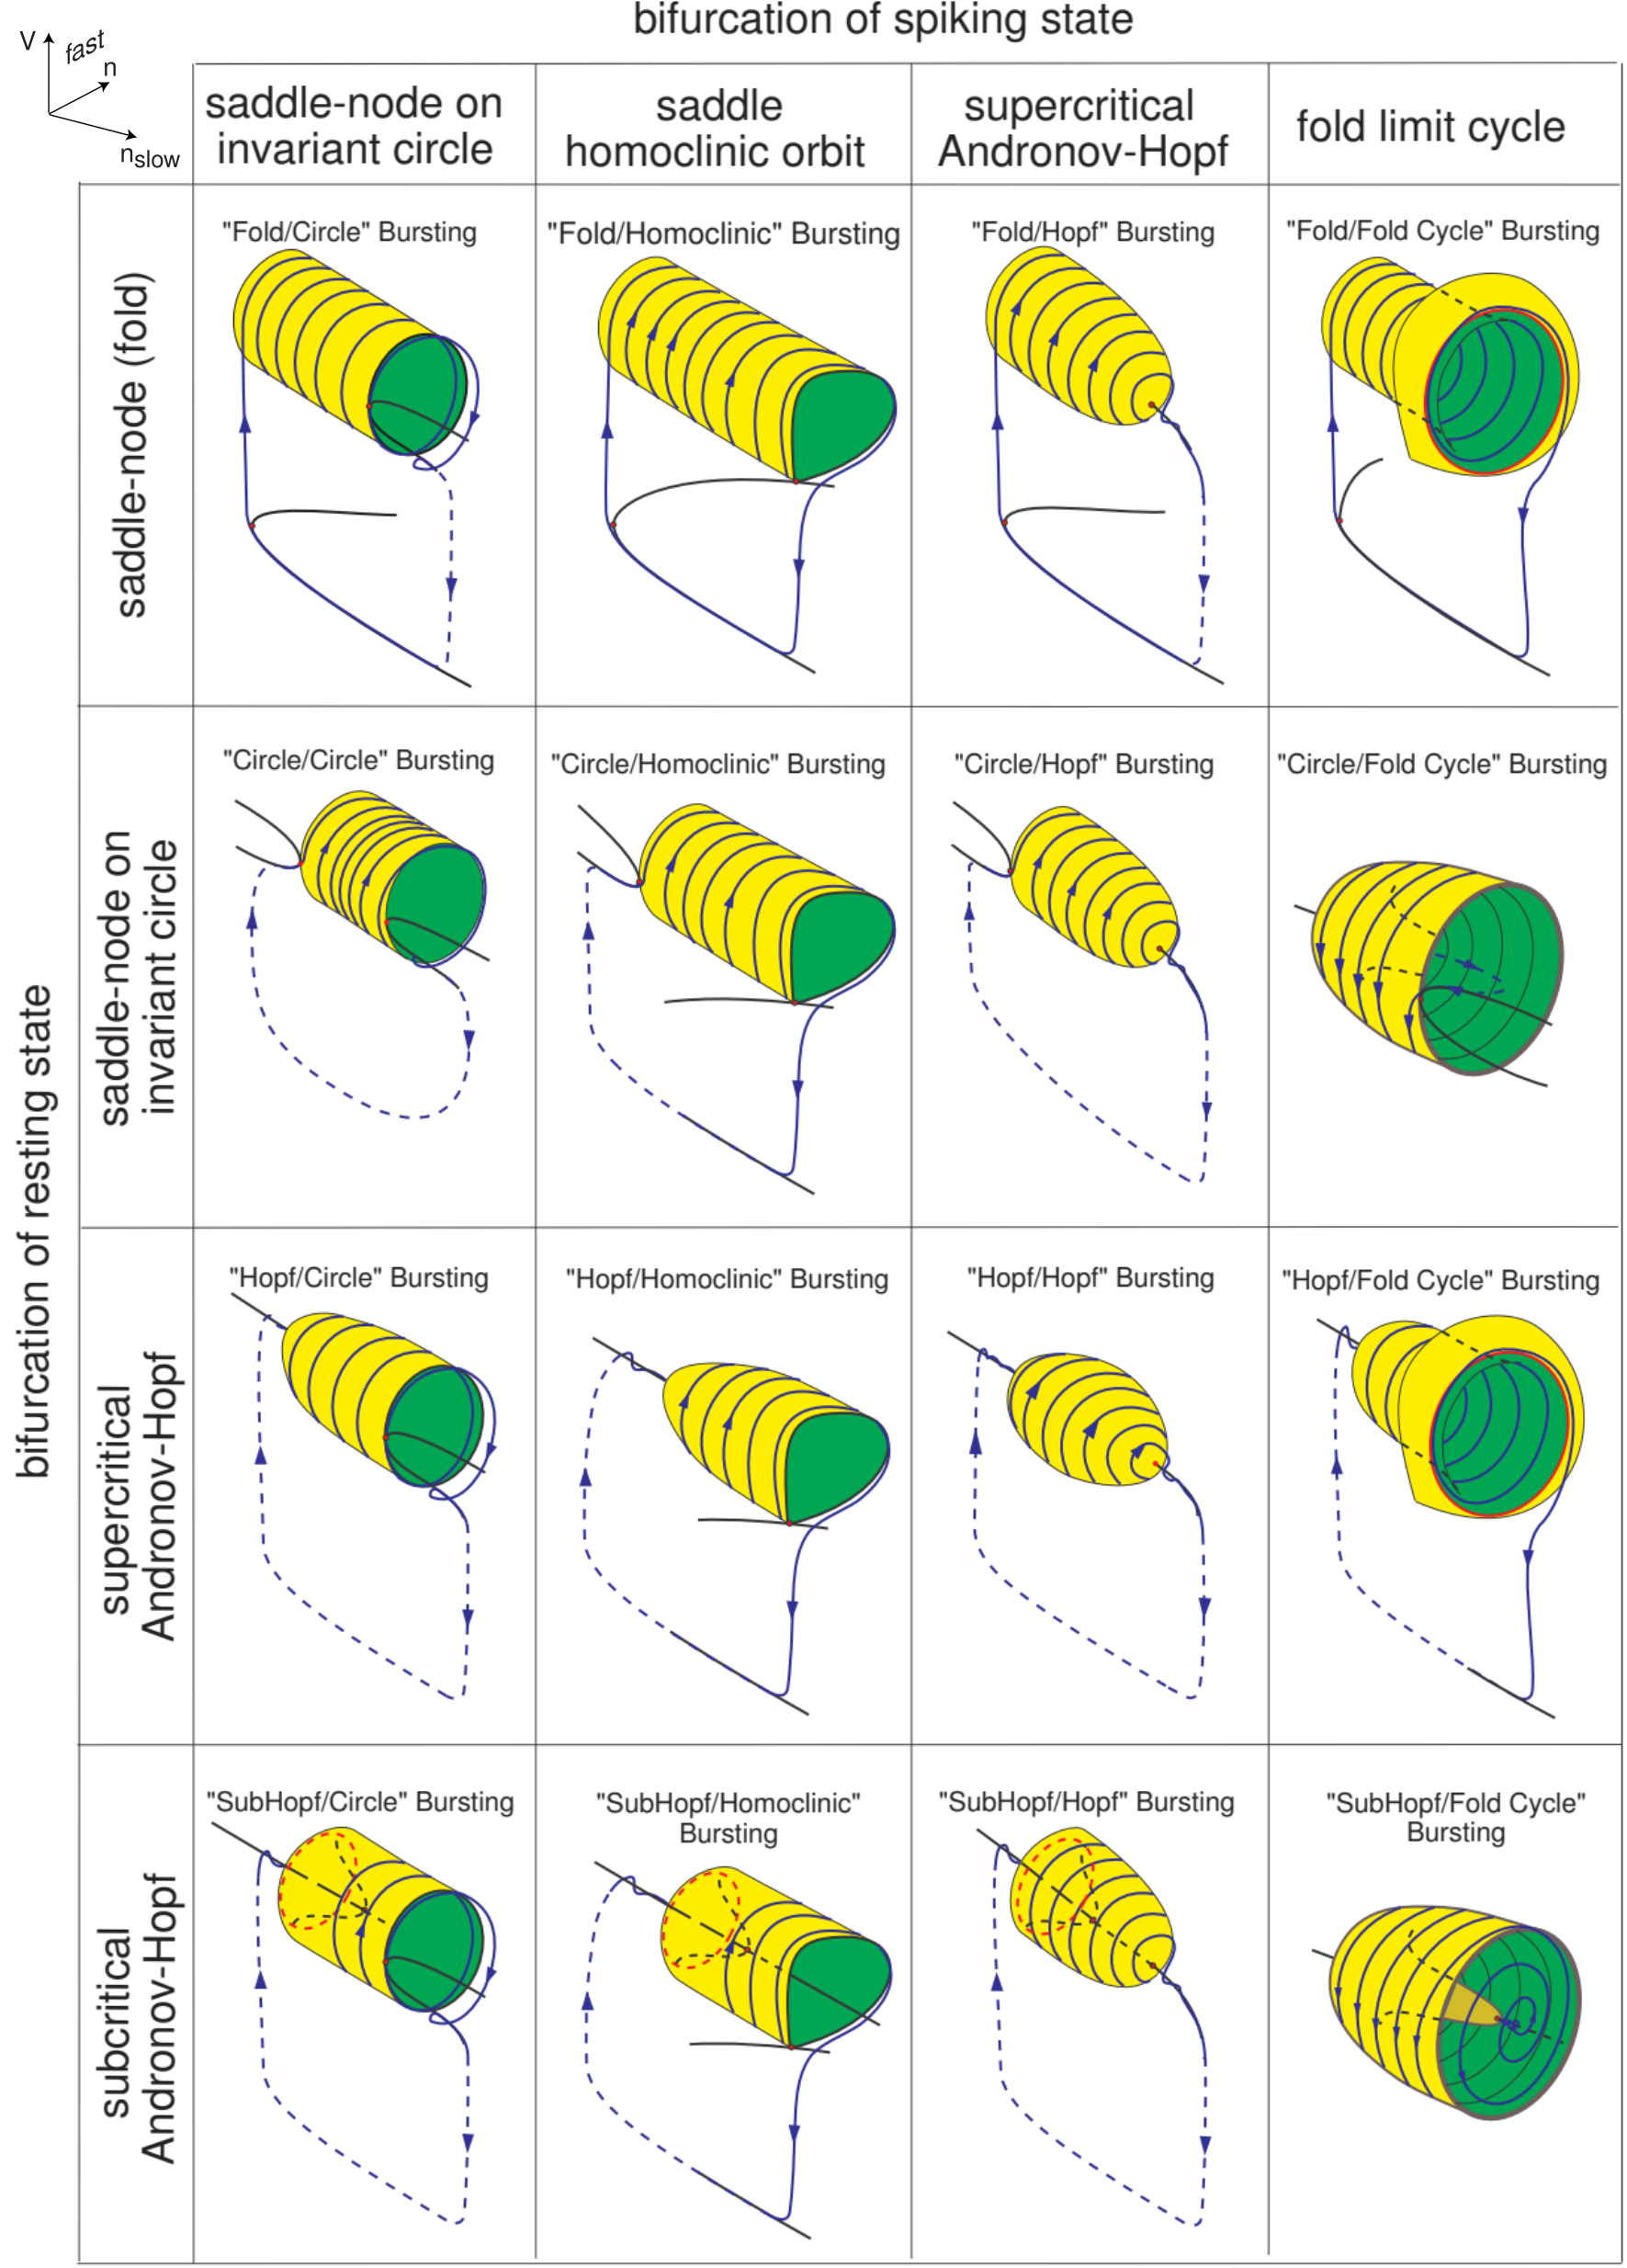
\includegraphics[width=0.75\linewidth]{../img/modeling_r5/examples/point_circle_bursters.png}
    \caption[Codimension-1 bifurcations of resting and spiking states for "2+1" point-circle bursters.]{
        Codimension-1 bifurcations of resting and spiking states for "2+1" point-circle bursters.
        The figure shows possible bifurcations for the case, when the fast (slow) system is
        two- (one-) dimensional. The inset on the top-left indicates the axis of the plots.
        $V$ - membrane potential, $n$ ($n_{slow}$) - fast (slow) variable of dynamical system.
        Adapted from \parencite{izhikevichDynamicalSystemsNeuroscience2006}, with modifications.
    }
    \label{fig:izhikevich_point_circle_bursters}
\end{figure}

\begin{figure}[!t]
    \centering
    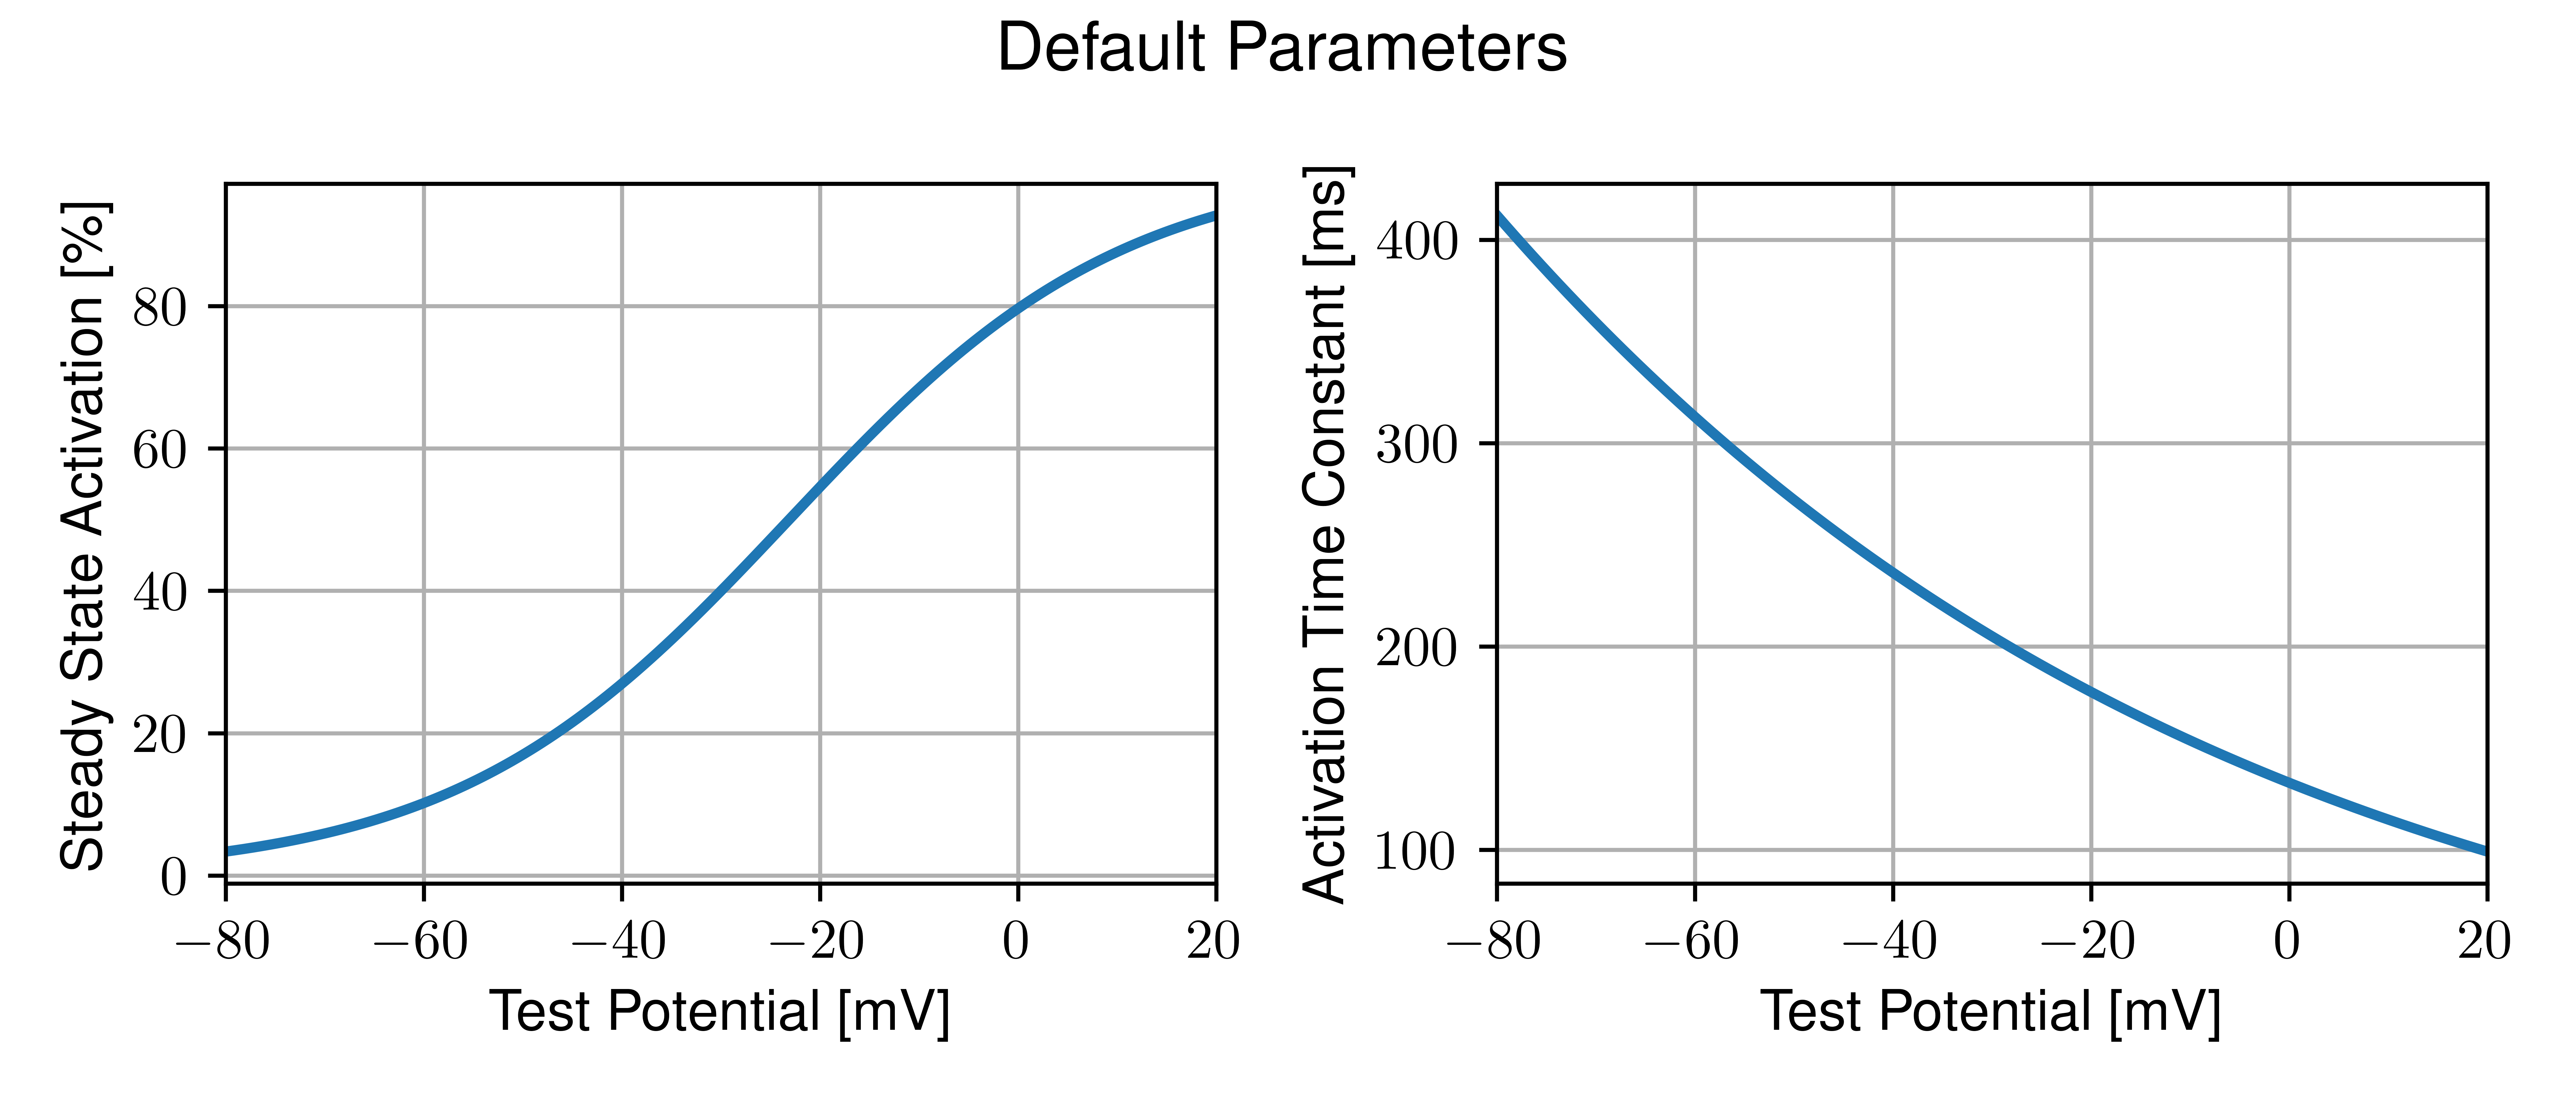
\includegraphics[width=0.85\linewidth]{../img/spiking_to_bursting/eag_default.png}
    \caption[EAG Channel Activation Variable and Kinetics]{
        \textbf{EAG Channel Activation Variable and Kinetics}. \textcolor{red}{TEXT!!!}
    }
    \label{fig:spiking_to_bursting_eag_params_default}
\end{figure}


\begin{figure}[!t]
    \centering
    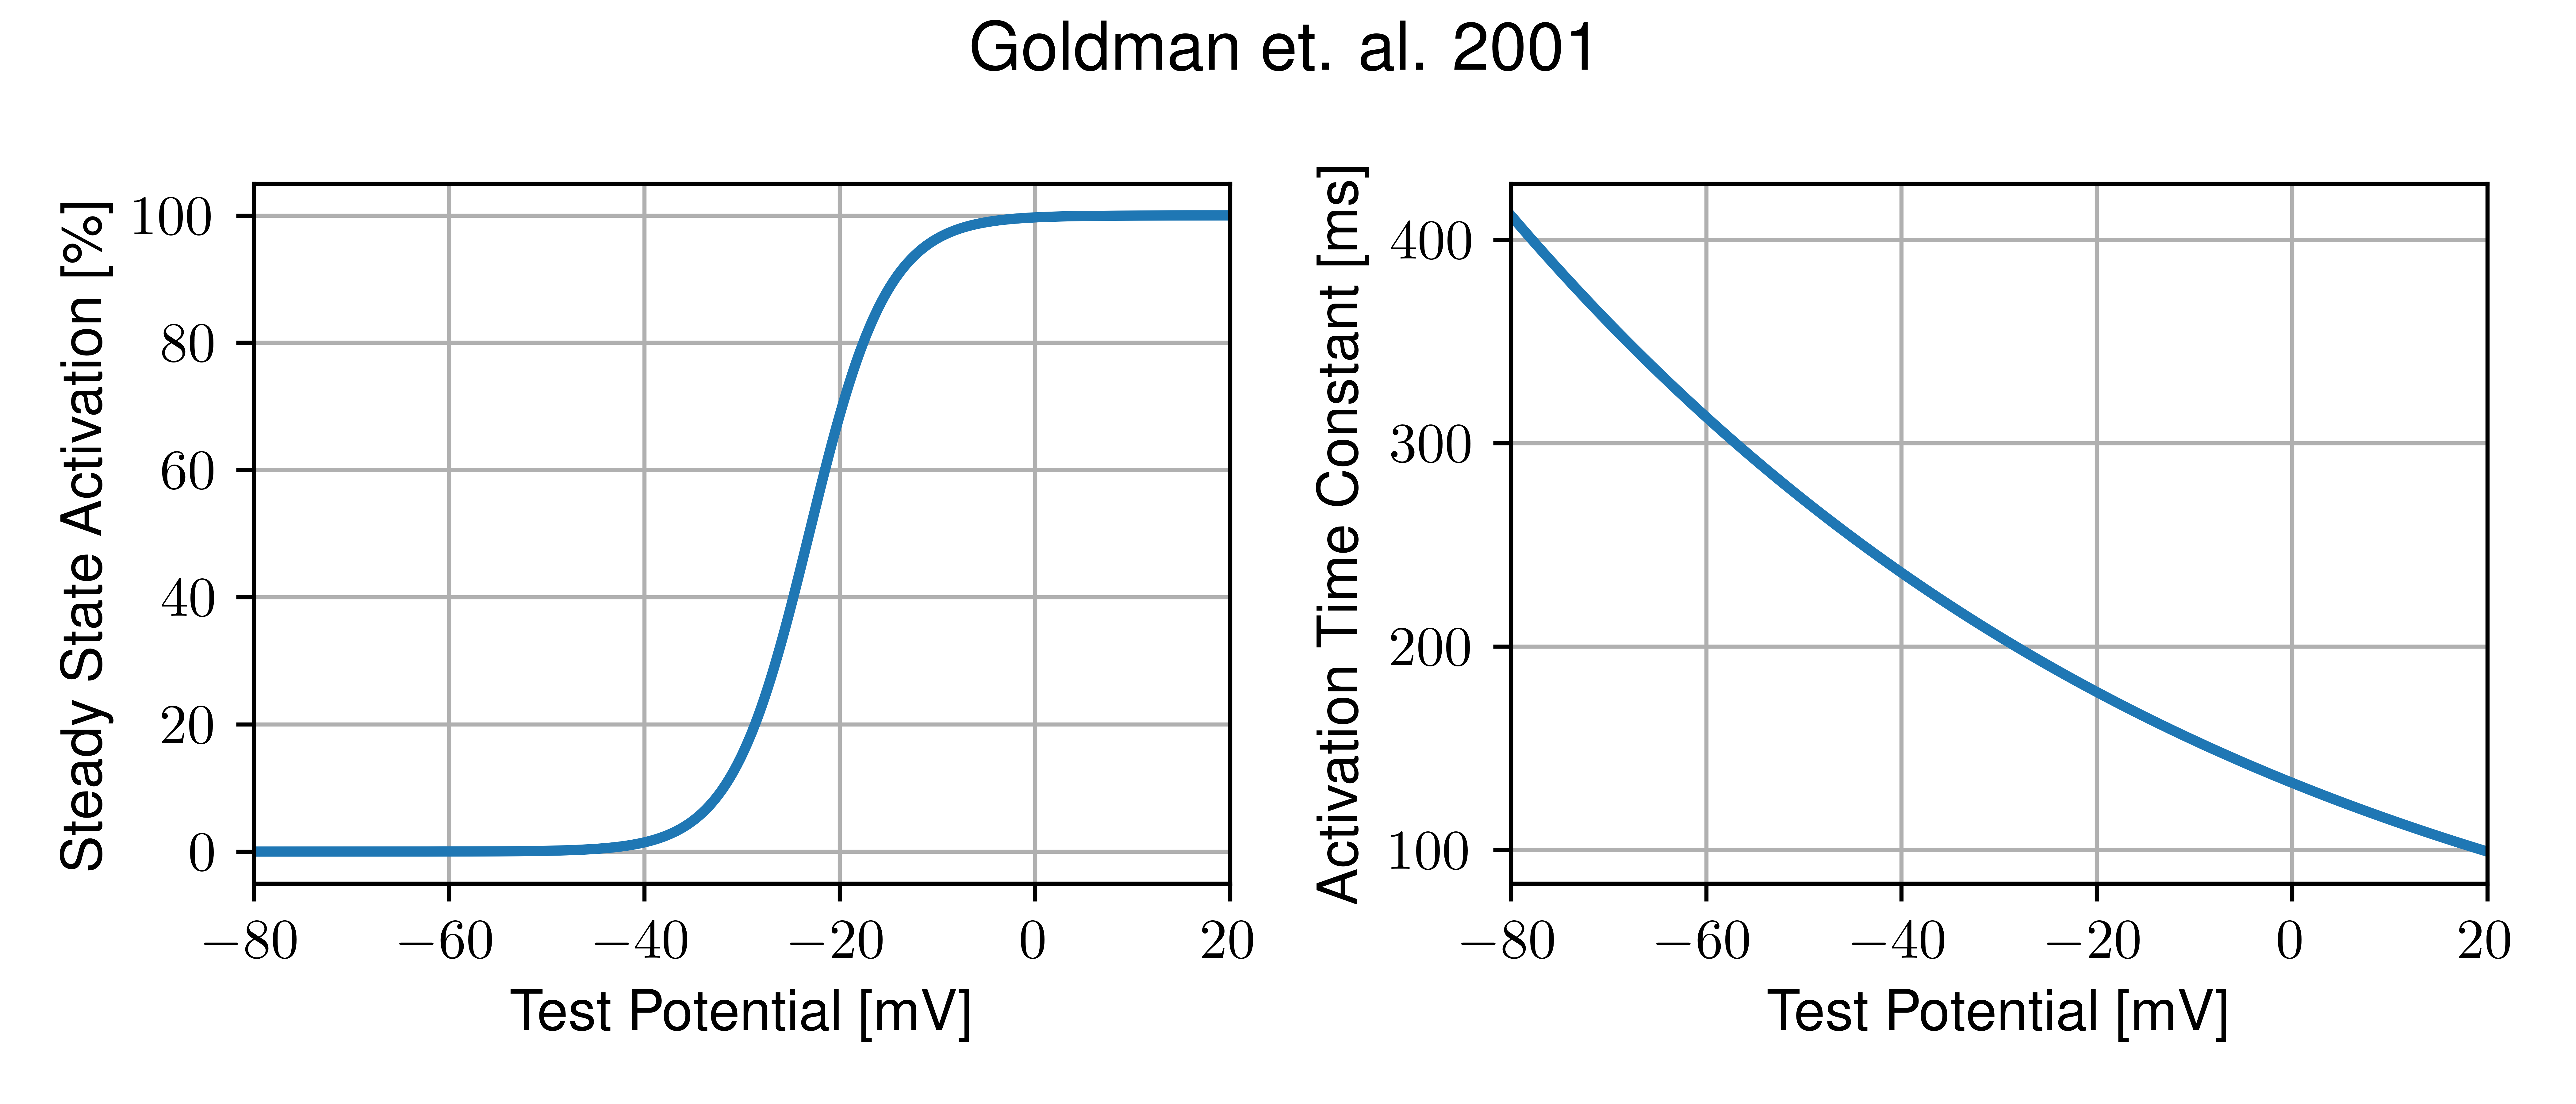
\includegraphics[width=0.8\linewidth]{../img/spiking_to_bursting/eag_goldman.png}
    \caption[EAG Channel Activation Variable and Kinetics for Goldman Model]{
        \textbf{EAG Channel Activation Variable and Kinetics for Goldman Model}. \textcolor{red}{TEXT!!!}
    }
    \label{fig:spiking_to_bursting_eag_params_goldman}
\end{figure}

\begin{figure}[!t]
    \centering
    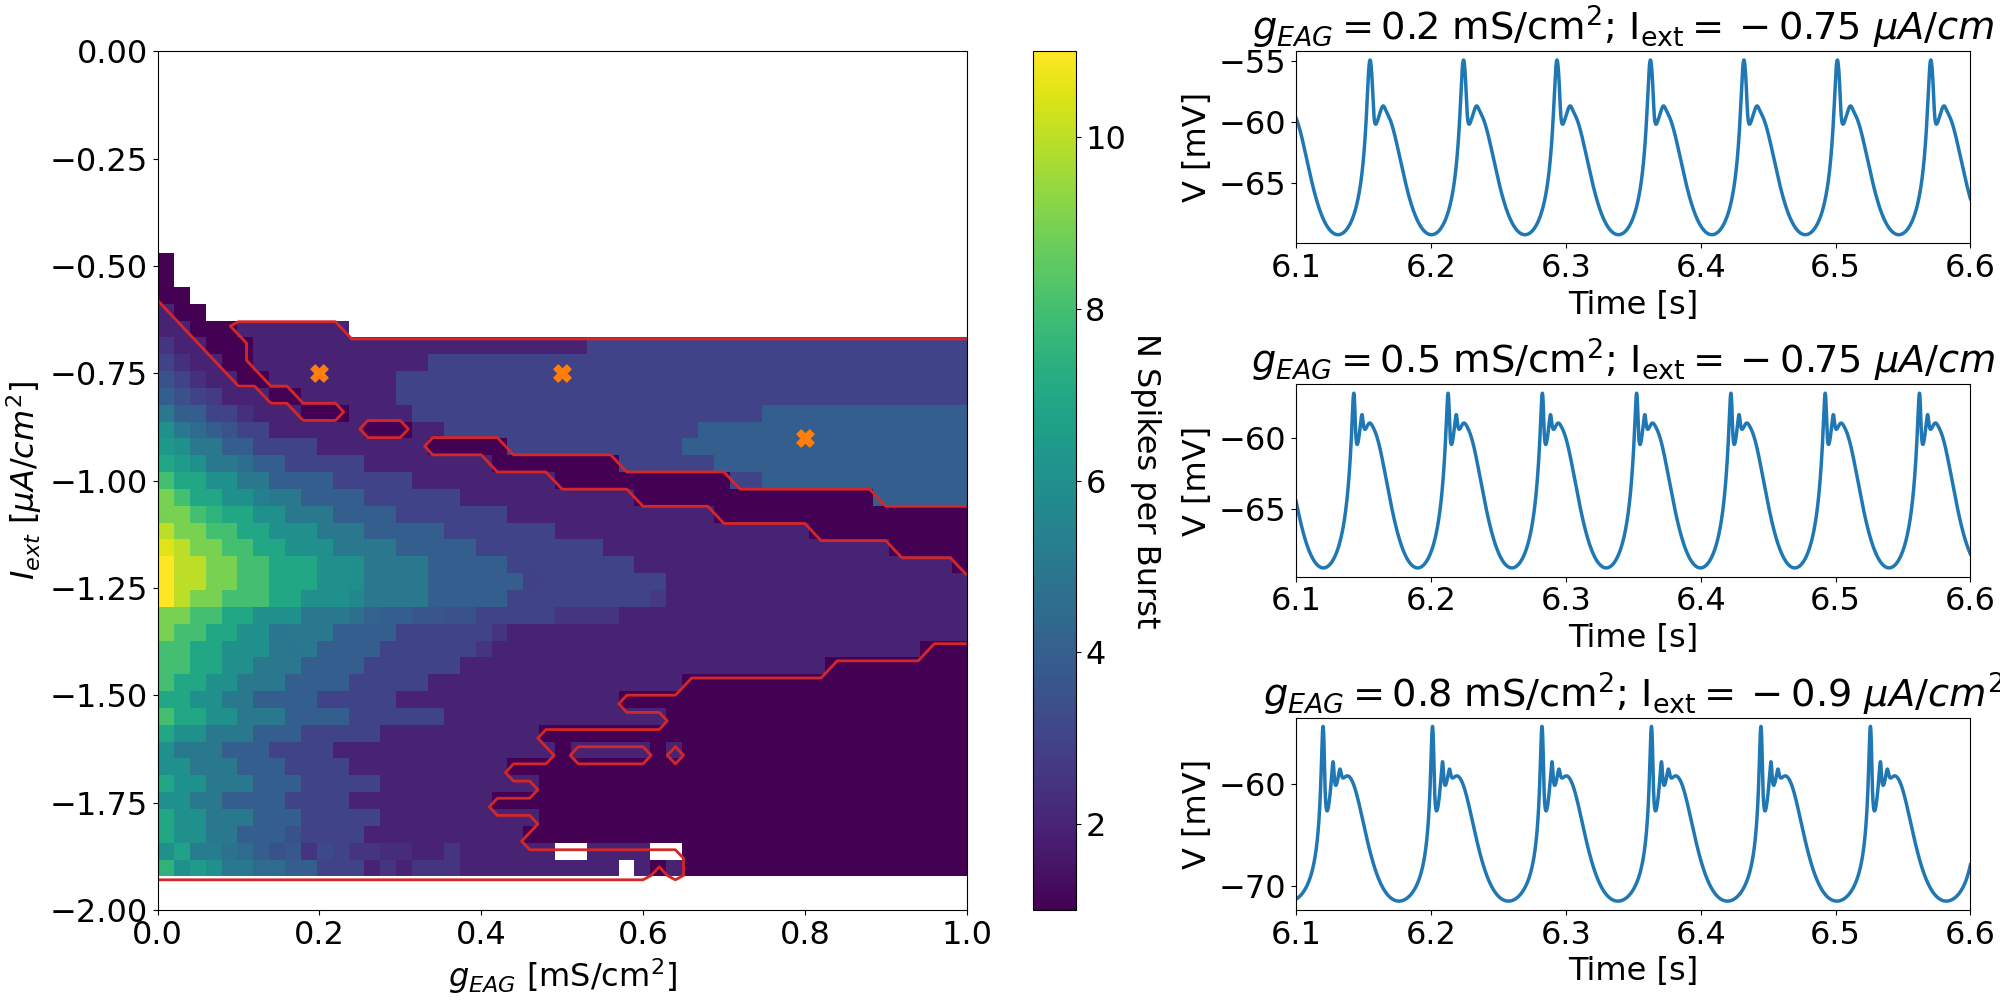
\includegraphics[width=\linewidth]{../img/spiking_to_bursting/nonlinearity_eag.png}
    \caption[Illustration of Methodological Limitation for Burst Detection]{
        \textbf{Illustration of Methodological Limitation for Burst Detection}. Burst detection was implemented as described in the supplementary material of \cite{franciRobustTunableBursting2018}. Left: same as Figure \ref{fig:spiking_to_bursting_wang_phase_diagram}. Right: Representative voltage traces obtained from simulations using the values of I$_{\text{ext}}$ and $g_{\text{EAG}}$ indicated by the orange 'x' markers on the heatmap.
    }
    \label{fig:nonlinearity_eag}
\end{figure}

\end{document}